\chapter{Beugung am Gitter}
\label{v:10}

In diesem Versuch benutzen Sie den Effekt der Beugung von Licht an einem optischen Gitter, um die Spektrallinien von Quecksilber zu betrachten, sowie die Wellenl"ange der gr"unen Linie zu messen.\\

%------------------------------------------------
\section{Stichworte}
%------------------------------------------------

Koh"arenz; Interferenz; Huygens'sches Prinzip; Gitterkonstante; Interferenzfilter; Beugung am Gitter.
%
%------------------------------------------------
\section{Literatur}
%------------------------------------------------

Gehrtsen, Kapitel 10.1.1-10.1.3, 10.1.12
%

%------------------------------------------------
\section{Anwendungsbeispiele}
%------------------------------------------------

Wann immer Licht durch eine endlich große Öffnung (Linse, Beleuchtungsspalt, etc) fällt, tritt an den Rändern dieser Öffnung Beugung auf. Diese begrenzt zum Beispiel das räumliche Auflösungsvermögen optischer Geräte oder des menschlichen Auges, ruft die Regenbogenmuster auf der beschriebenen Seite von CDs und den Halo um Sonne und Mond in dunstiger Atmosphäre hervor.\\
Beugung ist nicht auf Lichtwellen beschränkt, jede Art von Welle unterliegt dem Effekt. So kann zum Beispiel Schall das Ohr erreichen, auch wenn es keine direkte Sichtlinie zwischen Sprecher und Hörer gibt, oder Oberflächenwellen im Wasser erscheinen, obwohl der direkte Weg zum Verursacher der Wellen (vorbei fahrendes Schiff) versperrt ist.\\
Die Beugung von Erdbebenwellen kann benutzt werden, um Strukturuntersuchungen zwischen Erdkruste und Erdkern durchzuführen. Diese geben Auskunft über die Lage von Kohleflözen oder den Schalenaufbau der Erde.

%------------------------------------------------
\section{Theoretischer Hintergrund}
%------------------------------------------------

Die Kenntnis des Aufbaus der Atome gehört heute zu den gesicherten Bestandteilen von Physik und Chemie und ermöglicht ein Verständnis der Bindung in Molekülen und Festkörpern. Für die Aufklärung des Atombaus war die genaue Vermessung des von Atomen ausgesandten Lichtes von ganz wesentlicher Bedeutung.\\
Angeregte Atome senden Licht in Form von Spektrallinien aus, die für den Aufbau der äußeren Elektronenschalen und die chemischen Eigenschaften charakteristisch sind. Das einfachste Atom ist das Wasserstoffatom mit der bekannten Linienfolge der Balmerserie. Das im Periodensystem folgende Heliumatom besitzt zwei Elektronen, die wegen des
Elektronenspins auf verschiedene Weise koppeln können. Es ist interessant zu beobachten, dass das Spektrum der Spektrallinien des Quecksilberatoms mit seinen 80 Elektronen dem Spektrum des Heliumatoms in gewisser Weise ähnlich ist und dass man charakteristische Unterschiede auf die Relativitätstheorie zurückführen kann.\\
Das im Versuch vorgestellte Beugungsgitter ist ein einfaches, aber doch recht leistungsfähiges Gerät zur Sichtbarmachung von Spektrallinien und zur Vermessung von Wellenlängen, ein sogenanntes \textit{Spektrometer}.

\subsection{Interferenz}

Der Begriff der Interferenz bezeichnet die Überlagerung von zwei Wellenzügen. Je nachdem, ob die Auslenkung der beiden Wellen dasselbe Vorzeichen haben oder unterschiedliche, addieren oder subtrahieren sich ihre Auslenkungen zur überlagerten Welle. Man spricht dann von \textit{konstruktiver} oder \textit{destruktiver} Interferenz.\\
Damit ein sowohl räumlich (z.B. auf einem Schirm) als auch zeitlich stabiles Interferenzmuster entsteht, müssen die zwei oder mehr überlagerten Wellen \textit{kohärent} sein. Das ist dann der Fall, wenn die Zeitabhängigkeit der Amplitude in ihnen bis auf eine Phasenverschiebung die gleiche ist. Bei rein harmonischen Wellen (Sinus-förmig), wie z.B. Lichtwellen, heißt das, dass die Frequenzen übereinstimmen müssen; die Phasen dürfen eine konstante Differenz gegeneinander haben.\\
Beträgt die Phasendifferenz $\Delta$ ein ganzzahliges Vielfaches der Wellenlänge $\lambda$, findet konstruktive Interferenz statt:
\begin{equation}
	\Delta = n\cdot \lambda \quad\mathrm{mit}\, n= 0, 1, 2, ...
\end{equation}
Wellenberge treffen auf Wellenberge und Wellentäler auf Wellentäler, wodurch sich die Amplitude des resultierenden Strahls vergrößert und das Licht besonders hell erscheint.\\
Beträgt die Phasendifferenz hingegen ein halbzahliges Vielfaches der Wellenlänge,
\begin{equation}
	\Delta = \frac{2n+1}{2}\cdot \lambda \quad\mathrm{mit}\, n= 0, 1, 2, ...,
\end{equation}
so tritt destruktive Interferenz auf. Die Wellenberge und -täler heben sich ganz oder teilweise auf. Die Interferenz wirkt allerdings nur so lange, wie die Felder der Strahlen sich überlagern. Sie löscht das Licht nicht wirklich aus, und sobald sich die Strahlen voneinander entfernen, zeigen sie wieder ihre ursprüngliche Intensität.

\subsection{Beugung am Spalt}

Die Beugung von Licht an einem Spalt können Sie sich leicht mit dem Huygens'schen Bild der Elementarwellen klar machen. Betrachten Sie dabei jeden Punkt des Spaltes als Quelle von elementaren Kugelwellen, die sich in großem Abstand wieder zu einer ebenen Wellenfront überlagern. Zur Vereinfachung betrachten wir nur die Kugelwellen, die an den Kanten des Spaltes der Breite $d$ entstehen.\\
Betrachten Sie den Spalt unter einem Winkel $\alpha$, so müssen die Wellenfronten der beiden Seiten des Spaltes unterschiedlich lange Wege zurücklegen, um an Ihr Auge zu gelangen. Dieser \textit{Gangunterschied} beträgt, wie man Abbildung \ref{fig:Spalt} entnimmt:
\begin{equation}
 \Delta s = d\cdot\sin\alpha\, .
\end{equation}

\begin{figure}[ht]
	\centering
		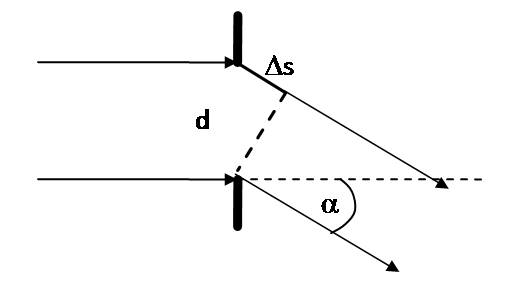
\includegraphics[width=.5\textwidth]{Abbildungen/Spalt.jpg}
	\caption{Beugung am Spalt}
	\label{fig:Spalt}
\end{figure}

\noindent
Beträgt der Gangunterschied ein ganzzahliges Vielfaches der Wellenlänge, so tritt konstruktive Interferenz auf, auf dem Schirm sieht man einen hellen Bereich, ein sog. \textit{Interferenzmaximum}. Mit der Definition des Gangunterschiedes ergibt sich also als Bedingung für die Beobachtung eines Interferenzmaximums:
\begin{equation} \label{eq:Interferenzmax}
 \sin\alpha_{max} = \frac{n\cdot\lambda}{d}\, .
\end{equation}
Den Faktor $n$ bezeichnet man die \textit{Ordnung des Maximums}.\\
Offenbar hängt die Richtung, unter der man ein Interferenzmaximum beobachtet, von der Wellenlänge des einfallenden Lichtes ab.

\subsection{Beugung am Gitter}

Ein (optisches) Gitter ist ein Anordnung aus vielen schmalen Spalten, die den (konstanten) Abstand $d$ voneinander haben. Die Anzahl der Spalten pro mm bezeichnet man als \textit{Gitterkonstante}.\\
Für die Beugung am Gitter gelten dieselben Überlegungen wie beim einzelnen Spalt (oder beim Doppelspalt). Mit Hilfe von Gleichung \ref{eq:Interferenzmax} kann man aus der Messung des Ablenkwinkels für das Maximum der $n$ten Ordnung die Wellenlänge bestimmen.
%den Abstand $\delta$ zwischen zwei Interferenzmaxima bestimmen. Wenn der Beobachtungsschirm im Abstand $L$ vom Spalt oder Gitter steht, so gilt 
%\begin{equation}\label{eq:10.1}
 %\frac{n\cdot\lambda}{d} = \sin\alpha = \frac{\delta}{L}\, .
%\end{equation}
%Diesen Zusammenhang kann man benutzen, um aus den messbaren Gr"o{\ss}en $L$ und $\delta$, mit Kenntnis der Gitterkonstante $d$, die Wellenlänge des einfallenden Lichtes zu messen:
%\begin{equation}
 %\lambda = \delta\cdot\frac{d}{L}\, .
%\end{equation}


%------------------------------------------------
\section{Fragen zur Vorbereitung}
%------------------------------------------------

\begin{enumerate}
 %
 %\item Was soll heute im Praktikum gemessen werden? Warum?
 %%
 \item Was besagt das Huygens'sche Prinzip?
 %
 \item Was ist Interferenz?
 %
 \item Welche Bedingungen m"ussen f"ur die Beobachtung von Interferenzerscheinungen erf"ullt sein?
 %
 \item Was bezeichnen die Gitterkonstante und der Gangunterschied?
 %
 \item Wird am Gitter rotes oder blaues Licht st"arker abgelenkt?
 %
 \item Welche Gr"o{\ss}e wird im Praktikum gemessen, welche Größe wird daraus berechnet?
 %
\end{enumerate}

%------------------------------------------------
\section{Durchführung} 
%------------------------------------------------

In diesem Versuch benutzen Sie denselben Aufbau wie in Versuch \ref{v:9}. Ersetzen Sie dabei nur das Prisma durch das optische Gitter.
\begin{enumerate}
	\item Stellen Sie die Hg-Cd Lampe vor den Beleuchtungsspalt und stellen Sie ein scharfes Abbild des Spaltes im Fernrohr ein. Stellen Sie dazu den Spalt so eng wie möglich.
	%
	\item Lesen Sie den Winkel auf dem Nonius ab und notieren ihn. 
	%
	\item Verschieben Sie das Fernrohr, bis das Spaltbild nicht mehr zu sehen ist. Anschließend zentrieren Sie das Bild des Spaltes wieder mithilfe des Fadenkreuzes und messen den Winkel erneut. Wiederholen Sie diesen Vorgang zwei Mal.
	%
	\item Stellen Sie nun das Gitter so auf den Teller des Goniometers, dass der Lichtstrahl möglichst senkrecht auf das Gitter fällt. \\
	\textbf{Fassen Sie dabei nicht das Gitter direkt an, da es sehr empfindlich ist!}\\
	Notieren Sie die auf dem Gitter angegeben Gitterkonstante.
	%
	\item Messen Sie nun die Ablenkwinkel der Spektrallinien der Hg-Cd Lampe für die Beugungsmaxima der ersten  und der zweiten Ordnung. 
\end{enumerate}
%------------------------------------------------
\section{Auswertung} 
%------------------------------------------------
\etodo{Musterauswertung}
\begin{enumerate}
	%
	\item Zeichnen Sie den Strahlengang und tragen Sie die gemessenen Winkel ein. Wie groß ist der Abstand $d$ zwischen zwei Gitterlinien?
 %
 %\item Berechnen Sie den Mittelwert $\overline{d}$ der Gitterkonstanten mitsamt seines Fehlers.
 %%
 %\item Tragen Sie die Stellung $x$ des Hebelarms in mm f"ur das $n$-te Maximum als Funktion der Ordnung $n$ auf. \label{aufg:gerade}
 %%
 %\item Berechnen Sie aus der Steigung der Geraden aus Aufgabe \ref{aufg:gerade}, mithilfe der Gitterkonstanten $\overline{g}$, die Wellenl"ange der gr"unen Hg-Linie.
  %\begin{itemize}
   %\item F"ur das Maximum der Ordnung $n$ gilt Gleichung \ref{eq:10.1}.
   %% 
   %\item Das Fernrohr ist auf einem Hebelarm der festen L"ange $l = 40$\,cm angebracht.
   %%
   %\item Aus der Stellung $x$ des Fernrohrs relativ zur Position des Hauptmaximums $x_0$ kann $\sin\alpha$ berechnet werden:
    %\begin{equation} \label{eq:10.2}
     %\sin\alpha = \frac{x-x_0}{l}
    %\end{equation}
    %Aus den Gleichungen \ref{eq:10.1} und \ref{eq:10.2} folgt
     %\begin{equation}
      %x = x_0 + \frac{l\cdot\lambda}{\overline{d}}n
     %\end{equation}
    %Dies ist eine Geradengleichung mit der Steigung $m=\frac{l\cdot\lambda}{\overline{d}}$.
   %%
   %\item Bestimmen Sie den Fehler der Wellenl"ange $\lambda$ mittels Fehlerfortpflanzung.
   %%
%  \end{itemize}
	\item Berechnen Sie die wirklichen Ablenkwinkel für die Beugungsmaxima.
	%
	\item Berechnen Sie die Standardabweichung des Mittelwertes aus den drei Messungen des Winkels, unter dem Sie das Spaltbild ohne Gitter betrachtet haben. Diese benutzen Sie als Ablesefehler für die folgenden Winkelmessungen.
	%
	\item Lösen Sie Gleichung \ref{eq:Interferenzmax} nach der Wellenlänge auf und benutzen Sie diese, um die Wellenlängen der Spektrallinien der Hg-Cd Lampe zu berechnen. Berechnen Sie ebenfalls die Unsicherheit auf die Wellenlänge. Machen Sie diese Berechnungen für die erste und zweite Ordnung getrennt.
	%
	\item Vergleichen Sie ihre Ergebnis mit den Literaturwerten in Tabelle \ref{tab:Wellenlaengen}. Diskutieren Sie Gründe für Abweichungen.
	%
\end{enumerate}

%\begin{table}[hb]
	%\centering
		%\begin{tabular}{l l l}
		%$\lambda$ in nm & rel. Int. & Farbe \\ \hline
		%623,44 & schwach & rot\\
		%579,06 & sehr stark & gelb \\
		%576.96 & sehr stark & gelb \\
		%546,07 & stark & gr"un \\	
		%491,60 & mittel & blaugr"un \\
		%435,84 & stark & blau \\
		%407,78 & mittel & violett \\
		%404,66 & mittel & violett \\
		%\end{tabular}
	%\caption{Die intensivsten Spektrallinien der Hg-Dampflampe}
	%\label{tab:SpektrallinienDerHgDampflampe}
%\end{table}